\documentclass[article]{ajs}

%%%%%%%%%%%%%%%%%%%%%%%%%%%%%%
%% declarations for jss.cls %%%%%%%%%%%%%%%%%%%%%%%%%%%%%%%%%%%%%%%%%%
%%%%%%%%%%%%%%%%%%%%%%%%%%%%%%

\usepackage{wrapfig}
\usepackage{graphicx}

%% almost as usual
\author{Sebastian Warnholz\\ Freie Universit\"at Berlin \And 
        Timo Schmid \\ Freie Universit\"at Berlin}
\title{Simulation Tools for Small Area Estimation: Introducing the \proglang{R}-package \proglang{saeSim}}

%% for pretty printing and a nice hypersummary also set:
\Plainauthor{Sebastian Warnholz, Timo Schmid} %% comma-separated
\Plaintitle{Simulation Tools for Small Area Estimation: Introducing the R-package saeSim} %% without formatting
\Shorttitle{Simulation Tools for Small Area Estimation} %% a short title (if necessary)

%% an abstract and keywords
\Abstract{
  The abstract of the article in English
  
}
\Keywords{package, small area estimation, reproducible research, simulation, \proglang{R}}
\Plainkeywords{package, small area estimation, reproducible research, simulation, R} %% without formatting
%% at least one keyword must be supplied

%% publication information
%% NOTE: Typically, this can be left commented and will be filled out by the technical editor
%% \Volume{50}
%% \Issue{9}
%% \Month{June}
%% \Year{2012}
%% \Submitdate{2012-06-04}
%% \Acceptdate{2012-06-04}
%% \setcounter{page}{1}
\Pages{1--xx}

%% The address of (at least) one author should be given
%% in the following format:
\Address{
  Sebastian Warnholz\\
  Department of Economics\\
  Freie Universit\"at Berlin\\
  D-14195 Berlin, Germany\\
  E-mail: \email{Sebastian.Warnholz@fu-berlin.de}\\
  URL: \url{http://www.wiwiss.fu-berlin.de/fachbereich/vwl/Schmid/Team/Warnholz.html}
}
%% It is also possible to add a telephone and fax number
%% before the e-mail in the following format:
%% Telephone: +43/512/507-7103
%% Fax: +43/512/507-2851

%% for those who use Sweave please include the following line (with % symbols):
%% need no \usepackage{Sweave.sty}

%% end of declarations %%%%%%%%%%%%%%%%%%%%%%%%%%%%%%%%%%%%%%%%%%%%%%%


\begin{document}
%
%% include your article here, just as usual
%
% R CMD Sweave %.Rnw
% Loading (and installing) necessary packages.
%
\section{Introduction}
Reproducible Research has become a widely discussed topic inside science and also the field of statistics. Thanks to the many mostly open-source tools like the \proglang{R}-language and \LaTeX, and also packages like knitr and Sweave, the integration of source code and text is possible and as a problem solved. In that sense the demand for Literate Programming can be if wanted incorporated in the work flow of a scientist. Not only are tools available to make research reproducible, also the demand of making the analysis of articles reproducible is rising. What this means is, that the source-code and data is published alongside an article. However, the requirements in style and clarity of source code are different from the written words in the article itself. This demand \textit{human readable source-code} has already been expressed by Knuth (1984): 
\begin{quote}
\textit{Instead of imagining that our main task is to instruct a computer what to do, let us concentrate rather on explaining to human beings what we want a computer to do.}
\end{quote}
Small Area Estimation is a growing field inside the field of statistics, where simulation studies play an important role. New statistical models are applied in model-based and design-based simulation studies. Considering the demands in reproducibility we want to propose a framework for simulation studies. This framework addresses three demands. First, making tools for data generation available and reusable. Second, unify the process behind simulation studies inside the field of Small Area Estimation. And third, making source-code of simulation studies available, such that it supports the conducted research in a transparent manner.
In this article we want to introduce a new package for the \proglang{R}-language addressing these demands. We will show the importance of simulation studies in the field. Introduce the simulation framework. And demonstrate how to use the package to map the simulation as a process to \proglang{R}.

\section{A simulation framework}
%
%% flow-diagram
\begin{wrapfigure}{R}{0.5\textwidth}
\begin{center}
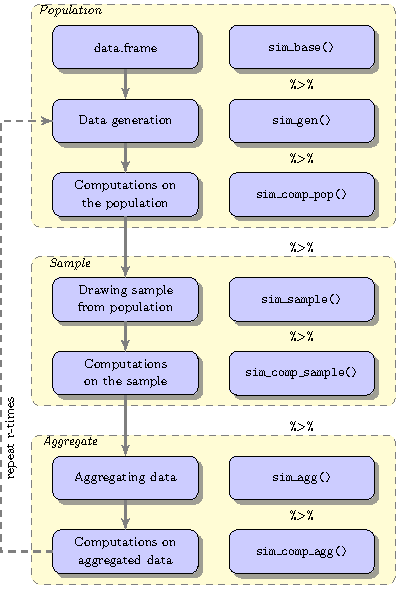
\includegraphics[width=0.5\textwidth]{flowdiagram}
\end{center}
\caption{\label{fig:flowdiagram}Process of simulation.} 
\end{wrapfigure}
%
In our opinion simulation studies can best be summarised when understood as a process of data manipulation. Thus the main focus of \proglang{saeSim} is to define the steps in that process which can then be \textit{cleanly} defined and repeated. Before we go into any detail of the functionality of the package we will discuss the process behind simulation studies and later how \proglang{saeSim} maps this process into \proglang{R}.

Simulation studies in small area estimation address three different levels, the population, the sample and data on aggregated level, as illustrated in figure \ref{fig:flowdiagram}. The \textbf{population-level} defines the data on which a study is conducted and may be a true population, synthetic population data or randomly generated variates from a model. We see three different point of views to define a population. First \textit{design-based}, which means that a simulation study is based on true or synthetic data of \textit{one} population. Second a \textit{semi-model-based} point of view, where only one population is drawn from a model and is fixed in the whole simulation study. And third, \textit{model-based} studies which have changing random populations drawn from a model.

The scope of this article is not not to promote any of those viewpoints, but simply to identify the similarity in them. The \textit{base} (first component in figure \ref{fig:flowdiagram}) of any simulation study is a data table, the question is, if this data is \textit{fixed} or \textit{random} over the course of the simulation. Or from a more technical point of view, is the data generation (the second step in figure \ref{fig:flowdiagram}) repeated in each simulation run or omitted?

Depending on the choice of a fixed or random population it is necessary to recompute the population domain-statistics like domain means and variances, or other statistics of interest (third component in figure \ref{fig:flowdiagram}).

The \textbf{sample-level} is when domain predictions are conducted for unit-level models. Independently of how the population is treated, fixed or random, this phase consists of two steps, first drawing a sample, and second conducting computations on the samples (fourth and fifth component in figure \ref{fig:flowdiagram}). Given a sample, design or model based small area methods are applied. Of interest are estimated parameters, which can be estimated model parameters or domain predictions as well as measures of uncertainty for the estimates.

As the sample-level is when unit-level models are applied, the \textbf{aggregate-level} is when area-level models are applied (the seventh and last component in figure \ref{fig:flowdiagram}). Area-level models in small area estimation typically only use information available for domains (in contrast to units). Thus, the question for simulation studies for area-level methods is, if the data is generated on unit-level and used after the aggregation (sixth component in figure \ref{fig:flowdiagram}) or if the data is generated directly on area-level, i.e. drawn from an area-level model. Depending on whether unit-level data and sampling are part of the simulation the aggregate-level follows the generation of the population or is based on the aggregated sample. Again, we do not promote a specific viewpoint but simply allow steps in the process of simulation to be omitted.

Depending on the topic of research steps in this simulation framework can be more relevant than others or completely irrelevant. We see these steps more as a complete list of phases one can encounter, thus single components can be omitted if not relevant in specific applications. For example \textit{data generation} is not relevant if you have population data, or the \textit{sample-level} is not used, when the sample is directly drawn from the model.

From this considerations, \proglang{saeSim} maps the different steps into \proglang{R}. Two layers with separate responsibilities need to be discussed. The first is \textit{how} different simulation components can be combined, and the second \textit{when} or in which order they are applied. Regarding the first, in \proglang{saeSim} we put a special emphasis on the interface of each component, which is to use functions which take a \proglang{data.frame} as argument and have a \proglang{data.frame} as return value. This is a widely used approach for data manipulation and promoted recently in the package \proglang{dplyr} \citep{wickham14}. This definition of interfaces, the return value of one component is the input of the next, is also used in \proglang{saeSim}.

Understanding a simulation as a process of manipulating one data object, see the second column in figure \ref{fig:flowdiagram} how the different steps in a simulation can be accessed. It is important to note that the functions in figure \ref{fig:flowdiagram} control the process, the second layer, i.e. \textit{when} components are applied. Each of these functions take a simulation setup object to be modified and a function with the discussed interface as arguments. Hence a simulation setup is a collection of functions to be applied in a certain sequence. As the first-layer functions, also have a defined interface: a \proglang{sim\_setup} as input to be modified and a \proglang{sim\_setup} as output. Thus, components can be chained together using the \textit{pipe operator} (\proglang{\%>\%}) from the package \proglang{magrittr} \citep{bache14}.

Braking the responsibility into what is applied and when it is applied addresses several aspects of reproducibility. First, by defining the interface between all components, it is easy to combine them in any combination and thus easy to share and reuse. Second, by controlling when components are applied we avoid the necessity of control structures in syntax and emphasise on the definition of components. The following example shows these aspects of the package using a predefined simulation setup:

\begin{Schunk}
\begin{Sinput}
> setup1 <- sim_base_lm() %>% sim_sample(sample_number(5))
> setup2 <- sim_base_lm() %>% sim_sample(sample_fraction(0.05))
\end{Sinput}
\end{Schunk}

Without knowing anything about the setup defined in \proglang{sim\_base\_lm} we can see that \proglang{setup1} and \proglang{setup2} only differ in the applied sampling scheme. \proglang{sim\_sample} is responsible to control when a function is applied (after the population-level) and \proglang{sample\_number(5)} and \proglang{sample\_fraction(0.05)} define the explicit way of drawing samples. The pipe operator \proglang{\%>\%} is used to add new components to the setup. As said before the composition of a simulation in that manner will focus on the definition of components and hide control structures. The next example will repeat the simulation stored in \proglang{setup1} two times. The results are returned in a list of \proglang{data.frame}s which have five rows as we sample 5 observations:

\begin{Schunk}
\begin{Sinput}
> setup1 %>% sim(R = 2) %>% sapply(nrow)
\end{Sinput}
\begin{Soutput}
[1] 5 5
\end{Soutput}
\end{Schunk}

With \proglang{saeSim} we want to contribute tools for simulation studies in the field of small area estimation. We see the need for sharing tools for data generation and simulation amongst the scientific community and thus defined an interface for these tools as well as designed a platform to make them accessible. By defining the steps behind a simulation we hope to promote a reasonable way to communicate them alongside publications and during research. In the next section we will present a case study and focus more on the concrete functionality provided by the package.

\section{Case study}

\section{Outlook}
Use this package to share and publish simulation studies alongside papers. Contribute to the package to make your ideas available. Contribute to the package and make your whole simulation study available. 


%\bibliographystyle{plainat}
\bibliography{saeSim}



\end{document}
